\section*{Math 202a - HW4 - Dan Davison - \texttt{ddavison@berkeley.edu}}
\begin{mdframed}
  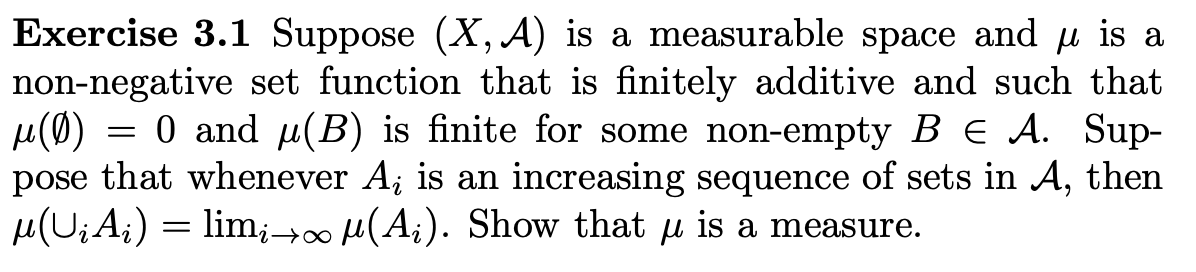
\includegraphics[width=400pt]{img/analysis--berkeley-202a-hw04-f604.png}
\end{mdframed}
\begin{claim*}
  $\mu$ is a measure.
\end{claim*}
\begin{proof}~\\
  It is given that $\mu$ is non-negative and that $\mu(\emptyset) = 0$. We must prove that $\mu$ is countably
  additive.

  So let $B_1, B_2, \dots$ be a pairwise disjoint countable collection of subsets of $X$. We want to show
  that $\mu(\bigcup_{i=1}^\infty B_i) = \sum_{i=1}^\infty \mu(B_i)$.

  Let's construct an increasing sequence of sets. Define $A_j = \bigcup_{i \leq j} B_i$ for $j=1, 2, \dots$, so
  that $A_1, A_2, \dots$ is an increasing sequence of sets. Note
  that $\bigcup_{i=1}^\infty B_i = \bigcup_{j=1}^\infty A_j$ therefore, by
  hypothesis,
  $\mu\big(\bigcup_{i=1}^\infty B_i\big) = \mu\big(\bigcup_{j=1}^\infty A_j\big) = \lim_{j\to\infty} \mu(A_j)$.

  Now, from finite additivity we have
  \begin{align*}
    \mu(A_j) = \mu(\bigcup_{i \leq j} B_i) = \sum_{i\leq j} \mu(B_i),
  \end{align*}
  therefore
  \begin{align*}
    \mu\big(\bigcup_{i=1}^\infty B_i\big) = \lim_{j\to\infty} \sum_{i\leq j} \mu(B_i) = \sum_{i=1}^\infty \mu(B_i),
  \end{align*}
  as required.
\end{proof}

\newpage
\begin{mdframed}
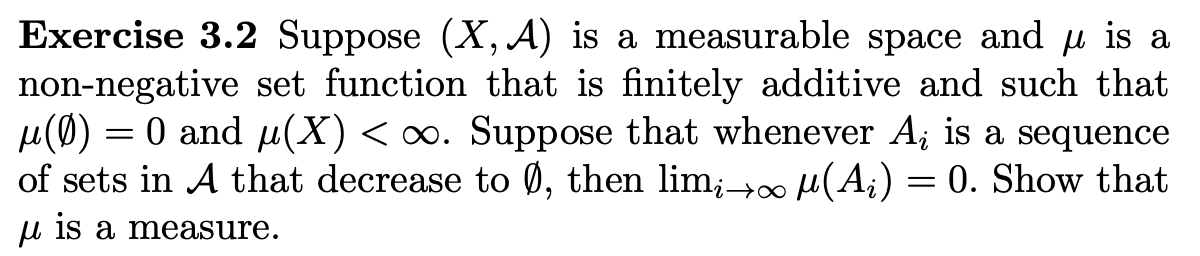
\includegraphics[width=400pt]{img/analysis--berkeley-202a-hw04-c187.png}
\end{mdframed}

\begin{proof}~\\

  \red{TODO}

  It is given that $\mu$ is non-negative and that $\mu(\emptyset) = 0$. We must prove that $\mu$ is countably
  additive.

  Let $A_1, A_2, \dots$ be a sequence of sets in $\mc A$ that decrease to $\emptyset$.

  Define $B_i = A_i \setminus \bigcup_{j > i} A_j = A_i \setminus A_{i+1}$. Then $B_1, B_2, \dots$ are a
  pairwise disjoint and countable collection of subsets of $X$. We want to show
  that $\mu(\bigcup_{i=1}^\infty B_i) = \sum_{i=1}^\infty \mu(B_i)$.

  We must use:
  \begin{enumerate}
  \item Finite additivity of $\mu$
  \item The fact that $\lim_{i\to\infty} \mu(A_i) = 0$.
  \end{enumerate}

  Morally, the result is true because some of the $B_i$ have non-zero measure, and yet their measure decreases
  to zero, and their sum is bounded above by $\mu(A_1)$.


  Note that $\bigcup_{i=1}^\infty B_i = \bigcup_{i=1}^\infty A_i = A_1$.

  From finite additivity we have that for all $n \in \N$
  \begin{align*}
    \mu(\bigcup_{i=1}^n B_i) = \sum_{i=1}^n \mu(B_i).
  \end{align*}
  Also



\end{proof}


\newpage
\begin{mdframed}
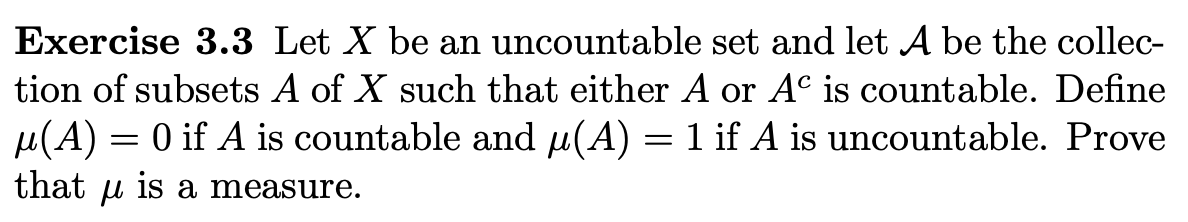
\includegraphics[width=400pt]{img/analysis--berkeley-202a-hw04-b168.png}
\end{mdframed}
\begin{proof}~\\
  $\emptyset$ is countable, therefore we have $\mu(\emptyset) = 0$ as required, and it remains to show
  that $\mu$ is countably additive.

  So let $B_1, B_2, \dots$ be a disjoint countable collection of subsets of $X$. We want to show
  that $\mu(\bigcup_{i=1}^\infty B_i) = \sum_{i=1}^\infty \mu(B_i)$.

  % Consider $\bigcup_{i=1}^\infty B_i$. It could be uncountable, since the $B_i$ could be a countable partition
  % of the entire set $X$. Could it also be countable? Yes, since the $B_i$ could be singletons. So we must
  % handle both cases.

  First suppose $\bigcup_{i=1}^\infty B_i$ is countable. Then no $B_i$ is uncountable. Therefore $\mu(B_i) = 0$
  for all $i$ and we have
  \begin{align*}
    \sum_{i=1}^\infty \mu(B_i) = \sum_{i=1}^\infty 0 = 0 = \mu\big(\bigcup_{i=1}^\infty B_i\big),
  \end{align*}
  as required.

  Next, suppose $\bigcup_{i=1}^\infty B_i$ is uncountable. We want to show
  that $\sum_{i=1}^\infty \mu(B_i) = 1$. Equivalently, we want to show that exactly one of the $B_i$ is
  uncountable. Note that $\ms A = \sigma(\ms A)$, and therefore we have by hypothesis that either $B_i$ is
  countable or $B_i^c$ is countable, for all $i$. Clearly some $B_i$ is uncountable or else we would
  have $\sum_{i=1}^\infty \mu(B_i) = \sum_{i=1}^\infty 0 = 0 \neq \mu\big(\bigcup_{i=1}^\infty B_i\big)$.
  Suppose for a contradiction that there exists $j \neq k$ such that $B_j$ and $B_k$ are uncountable. Note
  that $B_j$ and $B_k$ are disjoint, therefore $B_k \subseteq B_j^c$. But $B_j^c$ is countable, therefore $B_k$
  is countable; a contradiction. Therefore no such pair $j, k$ exists and we conclude that exactly one of
  the $B_i$ is uncountable, as required.
\end{proof}

\newpage
\begin{mdframed}
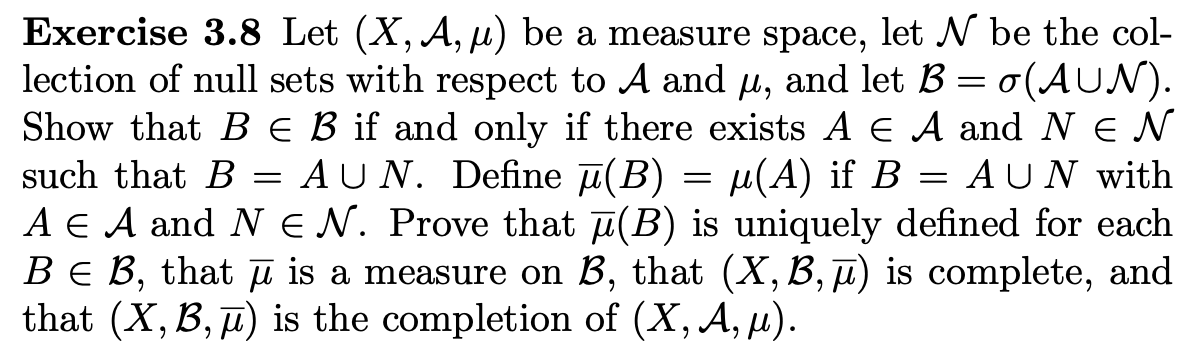
\includegraphics[width=400pt]{img/analysis--berkeley-202a-hw04-c88b.png}
\end{mdframed}

\begin{claim*}\label{claim-3-8-1}
  $B \in \mc B$ if and only if there exists $A \in \mc A$ and $N \in \mc N$ such that $B = A \cup N$.
\end{claim*}

\begin{proof}~\\
  Let $\mc B = \sigma(\mc A \cup \mc N)$ and let $\mc C$ be the collection of sets of the specified form,
  i.e. $\mc C = \{A \cup N ~:~ A \in \mc A, N \in \mc N\}$. We want to show that $\mc B = \mc C$.

  To show that $\mc C \subseteq \mc B$, let $A \in \mc A$ and $N \in \mc N$. Then $A \in \mc A \cup \mc N$,
  therefore $A \in \mc B$. And $N \in \mc A \cup \mc N$, therefore $N \in \mc B$.
  Therefore $C = A \cup N \in \mc B$.

  To show that $\mc B \subseteq \mc C$, first note that $\emptyset \in \mc A$ and $\emptyset \in \mc N$,
  therefore $\mc A \subset \mc C$ and $\mc N \subset \mc C$, therefore $\mc A \cup \mc N \subset \mc C$.

  We will show that $\mc C$ is a $\sigma$-algebra. Then, since $\mc A \cup \mc N \subset \mc C$, it follows
  that $\mc B := \sigma(\mc A \cup \mc N) \subseteq \sigma(\mc C) = \mc C$ as required.

  Since $\emptyset \in \mc A$ and $\emptyset \in \mc N$, we have $\emptyset \in \mc C$.

  Let $A \in \mc A$ and $N \in \mc N$. Then $(A \cup N)^C = A^c \cap N^c$. Since $A^c \in \mc A$
  and $N^c \in \mc N$, we see that $\mc C$ is closed under complements.

  It remains to show that $\mc C$ is closed under countable unions. So let $A_1, A_2, \dots \in \mc A$ and
  let $N_1, N_2, \dots \in \mc N$, and define $C_i = A_i \cup N_i$ for all $i$. Then
  \begin{align*}
    \bigcup_{i=1}^\infty C_i = \bigcup_{i=1}^\infty \big(A_i \cup N_i\big) = \big(\bigcup_{i=1}^\infty A_i\big) \bigcup \big(\bigcup_{i=1}^\infty N_i \big).
  \end{align*}
  Since $\big(\bigcup_{i=1}^\infty A_i\big) \in \mc A$ and $\big(\bigcup_{i=1}^\infty N_i\big) \in \mc N$ we see that $\big(\bigcup_{i=1}^\infty C_i\big) \in C$ as required.
\end{proof}

\begin{claim*}
  Define $\bar{\mu}(B) = \mu(A)$ if $B = A \cup N$ with $A \in \mc A$ and $N \in \mc N$.

  Then $\bar{\mu}(B)$ is uniquely defined for each $B \in \mc B$.
\end{claim*}

\begin{proof}~\\
  Let $A \in \mc A$ and $N \in \mc N$ and let $B = A \cup N \in \mc B$.

  Now let $A' \in \mc A$ and $N' \in N$ such that $B = A' \cup N'$.

  Without loss of generality, suppose that $A' \subseteq A$.

  We must show that $\bar{\mu}(A \cup N) = \bar{\mu}(A' \cup N')$. This is equivalent to showing
  that $\mu(A) = \mu(A')$.

  Note that $\mu(A) = \mu(A \cap A') + \mu(A \setminus A')$ and that $\mu(A') = \mu(A \cap A')$.

  We will show that $\mu(A \setminus A') = 0$. It will then follow that $\mu(A) = \mu(A \cap A') = \mu(A')$ as
  required.

  Let $n_1, n_2, \dots$ be indices of null sets in $\mc A$, so that $\mu(A_{n_i}) = 0$ for all $i$.

  Note that since $N$ is a null set, there exists $A_{n_i} \in \mc A$ such that $N \subseteq A_{n_i}$
  and $\mu(A_{n_i}) = 0$. Similarly, there exists $A_{n_j} \in \mc A$ such that $N' \subseteq A_{n_j}$
  and $\mu(A_{n_j}) = 0$.

  Let $A_{n_k} = A_{n_i} \cup A_{n_j}$. Note that $\mu(A_{n_k}) = 0$
  since $\mu(A_{n_k}) \leq \mu(A_{n_i}) + \mu(A_{n_j}) = 0 + 0 = 0$.

  Now, we have $A \subseteq B \subseteq A' \cup A_{n_k}$.

  Therefore, since $A' \subseteq A$, we have
  \begin{align*}
        &(A \cap A') \cup (A \setminus A') \subseteq (A \cap A') \cup A_{n_k} \\
    \iff &(A \setminus A') \subseteq A_{n_k}.
  \end{align*}
  Therefore
  \begin{align*}
    \mu(A \setminus A') \leq \mu(A_{n_k}) = 0,
  \end{align*}
  therefore $\mu(A \setminus A') = 0$ as required.
\end{proof}

\begin{claim*}
  $\bar{\mu}$ is a measure on $\mc B$.
\end{claim*}

\begin{proof}~\\
  Since $\emptyset \in \mc A$ and $\emptyset \in \mc N$ we
  have $\bar\mu(\emptyset) = \bar\mu(\emptyset \cup \emptyset) = \mu(\emptyset) = 0$ as required.

  It remains to show that $\bar\mu$ is countably additive on $\mc B$. So let $B_1, B_2, \dots \in \mc B$ be
  countable and pairwise disjoint where for each $i$ these decompose as $B_i = A_i \cup N_i$
  with $A_i \in \mc A$ and $N_i \in \mc N$. Note that, since the $B_i$ are pairwise disjoint, so the $A_i$ are
  pairwise disjoint (and also the $N_i$). Then
  \begin{align*}
    \bar\mu\Big(\bigcup_{i=1}^\infty B_i\Big)
    = \bar\mu\Big(\bigcup_{i=1}^\infty (A_i \cup N_i)\Big)
    = \bar\mu\Big(\bigcup_{i=1}^\infty A_i ~\cup~ \bigcup_{i=1}^\infty N_i\Big).
  \end{align*}
  Therefore, since $\bigcup_{i=1}^\infty A_i \in \mc A$ and $\bigcup_{i=1}^\infty N_i \in \mc N$,
  \begin{align*}
    \bar\mu\Big(\bigcup_{i=1}^\infty B_i\Big)
    = \mu\Big(\bigcup_{i=1}^\infty A_i\Big)
    = \sum_{i=1}^\infty \mu(A_i)
    = \sum_{i=1}^\infty \bar\mu(B_i),
  \end{align*}
  as required.
\end{proof}

\begin{claim*}
  $(X, \mc B, \bar{\mu})$ is complete.
\end{claim*}

\begin{proof}~\\
  By definition, $(X, \mc B, \bar{\mu})$ is complete if all null sets with respect to $\bar\mu$ and $\mc B$ are
  in $\mc B$.

  Let $N_1$ be a null set with respect to $\bar\mu$ and $\mc B$. Then there exists $B_1 \in \mc B$
  with $\bar\mu(B_1) = 0$ such that $N_1 \subseteq B_1$.

  Since $B_1 \in \mc B$ it is of the form $B_1 = A_1 \cup N_2$ where $A_1 \in \mc A$ and $N_2 \in \mc N$. Therefore
  $N_1 \subseteq A_1 \cup N_2$.

  Furthermore, since $N_2 \in \mc N$, there exists $A_2 \in \mc A$ such that $N_2 \subseteq A_2$.
  Therefore $N_1 \subseteq A_1 \cup A_2$.

  But then $N_1 \in \mc N$, hence $N_1 \in \mc B$ as required.
\end{proof}

\begin{claim*}
  $(X, \mc B, \bar{\mu})$ is the completion of $(X, \mc A, \mu)$.
\end{claim*}

\begin{proof}~\\
  We've already shown that $(X, \mc B, \bar\mu)$ is complete with $\bar{\mu}$ an extension of $\mu$. It remains
  to show that no smaller $\sigma$-algebra exists that is complete with respect to its associated measure.

  Let $(X, \mc B', \mu')$ be complete, with $\mu'$ an extension of $\mu$. Let $A \cup N \in \mc B$,
  where $A \in \mc A$ and $N \in \mc N$.

  Suppose for a contradiction that $A \cup N \notin \mc B'$.

  What is the contradiction? It could be that $(X, \mc B', \mu')$ is not complete, or that $\mu'$ is not an
  extension of $\mu$.

  \red{TODO}
\end{proof}

\newpage
\begin{mdframed}
  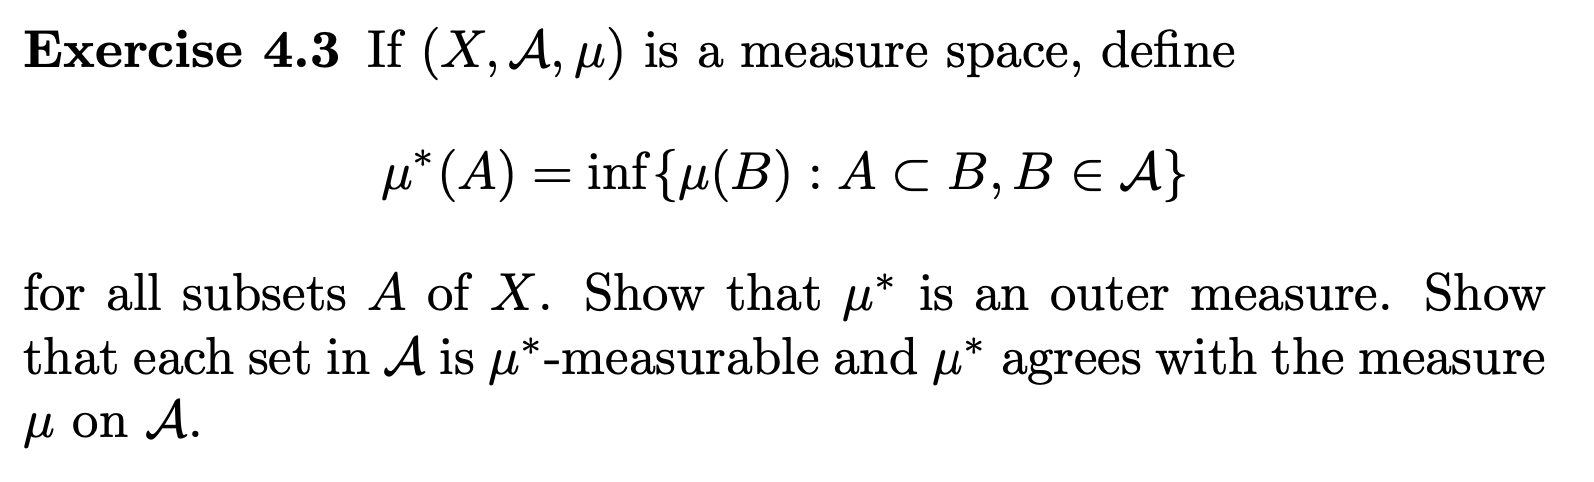
\includegraphics[width=400pt]{img/analysis--berkeley-202a-hw-0d98.png}
\end{mdframed}

\begin{claim*}
  $\mu^*$ is an outer measure.
\end{claim*}

\begin{proof}~\\
  Note that $\mu^*(\emptyset) = 0$, since $\emptyset$ is covered by $\emptyset \in \mc A$ with $\mu(\emptyset) = 0$.

  It remains to show that $\mu^*$ is countably sub-additive.

  Let $A_1, A_2, \dots \in X$. We must show that
  \begin{align*}
    \mu^*\Big(\bigcup_{i=1}^\infty A_i\Big) \leq \sum_{i=1}^\infty \mu^*(A_i).
  \end{align*}
  Note that $X \in \mc A$, therefore every $A_i$ is a subset of some set in $\mc A$.

  Let $\epsilon > 0$. For $i \in \N$, let $C_i \in \mc A$ be such that $A_i \subseteq C_{i}$ with
  \begin{align*}
    \mu(C_{i}) < \mu^*(A_i) + \epsilon/2^i.
  \end{align*}
  (We can do this because $\mu^*(A_i)$ is defined as an infimum over covering sets; if for some $\epsilon_i$
  there did not exist a $C_i$ such that $\mu(C_{i}) < \mu^*(A_i) + \epsilon_i$ then $\mu^*(A_i) + \epsilon_i$
  would be a lower bound; a contradiction.)

  Then we have
  \begin{align*}
    \mu^*\Big(\bigcup_{i=1}^\infty A_i\Big) \leq \sum_{i=1}^\infty \mu(C_{i}) < \sum_{i=1}^\infty \mu^*(A_i) + \epsilon.
  \end{align*}
  Since $\eps > 0$ is arbitrary, this implies
  \begin{align*}
    \mu^*\Big(\bigcup_{i=1}^\infty A_i\Big) \leq \sum_{i=1}^\infty \mu^*(A_i),
  \end{align*}
  as required.
\end{proof}






















\begin{claim*}
  Each set in $\mc A$ is $\mu^*$-measurable.
\end{claim*}

\begin{proof}~\\
  Let $B \in \mc A$. We must show that
  \begin{align*}
    \mu^*(B) = \mu^*(B \cap E) + \mu^*(B \cap E^c),
  \end{align*}
  for every $E \subseteq X$.

  So let $E \subseteq X$. Note that
  \begin{align*}
    \mu^*(B) \leq \mu^*(B \cap E) + \mu^*(B \cap E^c).
  \end{align*}
  is a statement of finite sub-additivity of $\mu^*$, which follows from countable sub-additivity of $\mu^*$
  (form a countable sequence with $B_1 = B \cap E$, $B_2 = B \cap E^c$, and $B_i = \emptyset$ for $i > 2$ and
  apply countable additivity), so what remains to prove is that
  \begin{align*}
    \mu^*(B) \geq \mu^*(B \cap E) + \mu^*(B \cap E^c).
  \end{align*}
  Fix $\eps > 0$ and let $C_{1}, C_{2}, \dots \in \mc A$ be such that $B \subseteq \bigcup_{i=1}^\infty C_{i}$ with
  \begin{align*}
    \sum_{i=1}^\infty C_i < \mu^*(B) + \eps.
  \end{align*}
  Then
  \begin{align*}
    \mu^*(B) + \eps
    &> \sum_{i=1}^\infty \mu(C_i) \\
    &= \sum_{i=1}^\infty \mu(C_i \cap E) + \sum_{i=1}^\infty \mu(C_i \cap E^c) \\
    &\geq \mu(B \cap E) + \mu(B \cap E^c).
  \end{align*}
  Since $\eps$ is arbitrary it follows that
  \begin{align*}
    \mu^*(B) \geq \mu^*(B \cap E) + \mu^*(B \cap E^c),
  \end{align*}
  as required.
\end{proof}

\begin{claim*}
  $\mu^*$ agrees with the measure $\mu$ on $\mc A$.
\end{claim*}

\begin{proof}~\\
  Let $B \in \mc A$ and let $\mc B = \{B' : B \subseteq B', B' \in \mc A\}$. We must show
  that $\mu^*(B) = \mu(B)$. We have
  \begin{align*}
    \mu^*(B)
    &:= \inf \{\mu(B') : B' \in \mc B\} \\
    &=  \inf \{\mu(B \cup (B' \setminus B)) : B' \in \mc B\} \\
    &=  \inf \{\mu(B) + \mu(B' \setminus B) : B' \in \mc B\}.
  \end{align*}
  Let $M = \{\mu(B) + \mu(B' \setminus B) : B' \in \mc B\}$; the set over which this last infimum is taken.
  Note that $B \in \mc B$, therefore $\mu(B) = \mu(B) + \mu(\emptyset) \in M$. Furthermore, since $\mu$ is
  non-negative, $m \geq \mu(B)$ for all $m \in M$. Therefore $\mu(B)$ is a minimum of $M$, and therefore it is
  the infimum of $M$, as required.
\end{proof}

\newpage
\begin{mdframed}
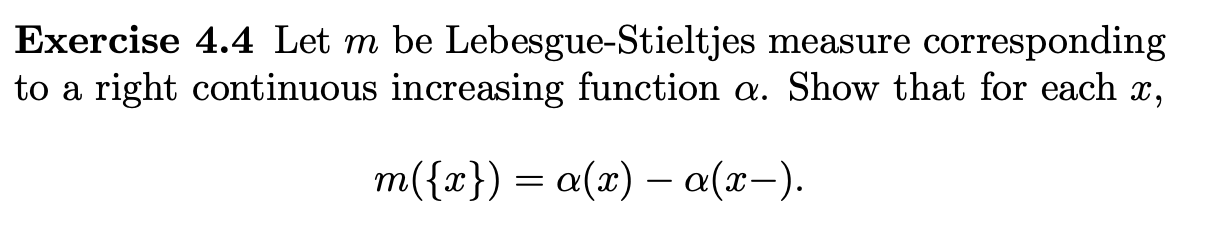
\includegraphics[width=400pt]{img/analysis--berkeley-202a-hw04-c0b6.png}
\end{mdframed}

\begin{proof}~\\
  By definition,
  \begin{align*}
    m(\{x\}) := \inf \Big\{\sum_{i=1}^\infty l(I_i) : \Big\}
  \end{align*}

\end{proof}




























\begin{comment}
\newpage
  EXERCISE 3.3 FROM OLD VERSION
  \begin{mdframed}
    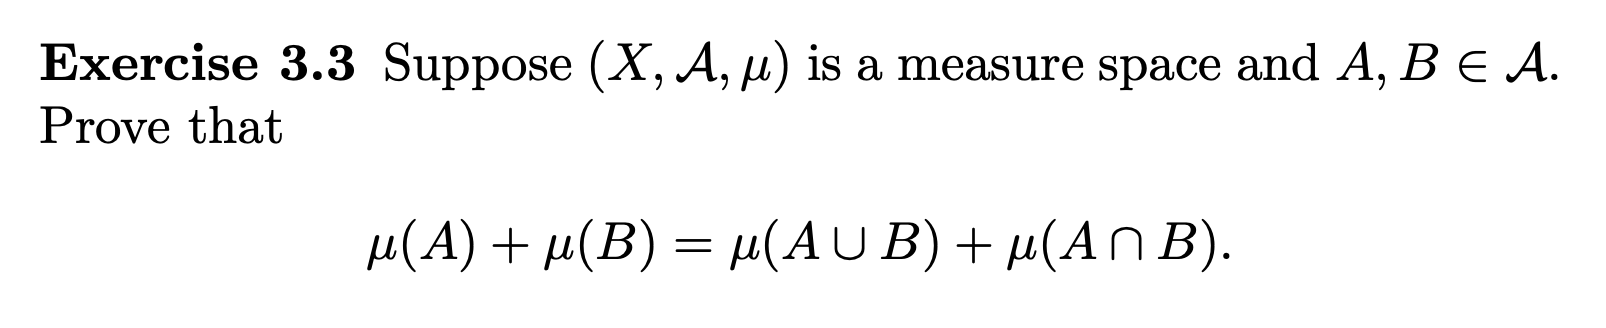
\includegraphics[width=400pt]{img/analysis--berkeley-202a-hw-2389.png}
  \end{mdframed}

  \begin{proof}~\\
    From finite additivity we have
    \begin{align*}
      \mu(A \cup B) &= \mu(A) + \mu(A \setminus B). \\
      \mu(A \cup B) &= \mu(B) + \mu(B \setminus A).
    \end{align*}
    Summing these gives
    \begin{align*}
      2\mu(A \cup B)
      = \mu(A) + \mu(B) + \mu(A \triangle B)
    \end{align*}
    But $\{A \triangle B, A \cap B\}$ is a partition of $A \cup B$ hence from finite additivity
    again $\mu(A \triangle B) + \mu(A \cap B) = \mu(A \cup B)$. Therefore
    \begin{align*}
      2\mu(A \cup B) = \mu(A) + \mu(B) + \mu(A \cup B) - \mu(A \cap B),
    \end{align*}
    or equivalently
    \begin{align*}
      \mu(A \cup B) = \mu(A) + \mu(B) - \mu(A \cap B).
    \end{align*}
  \end{proof}

  \begin{mdframed}
    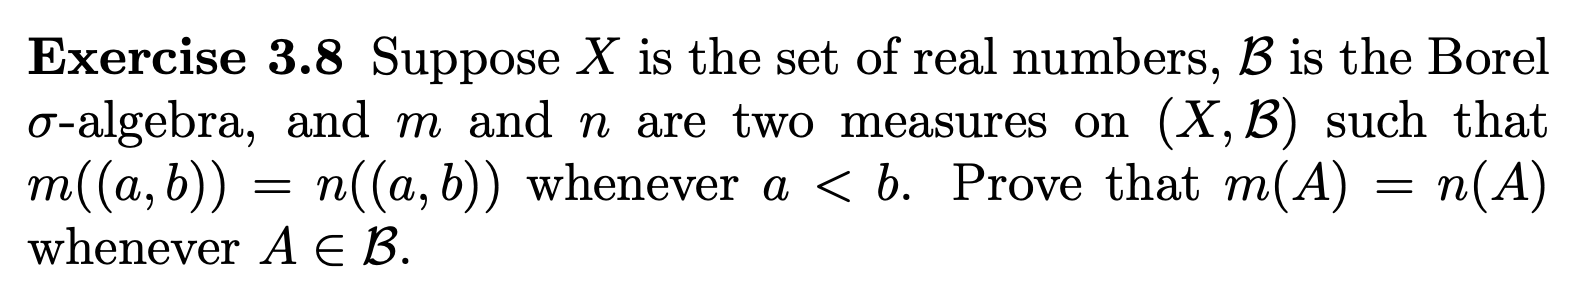
\includegraphics[width=400pt]{img/analysis--berkeley-202a-hw-3a79.png}
  \end{mdframed}

  \begin{claim*}
    If $m$ and $n$ have the same value on any open interval in $B$ then they have the same value on any set
    in $\mc B$.
  \end{claim*}

  \begin{proof}~\\
    Let $\mc O$ be the collection of open subsets of $\R$.

    Let $O \in \mc O$. Then $O$ can be written as a countable union of disjoint open intervals, $O = \bigcup_i I_i$. Therefore
    \begin{align*}
      m(O) = m(\bigcup_i I_i) = \sum_i m(I_i) = \sum_i n(I_i) = n(O).
    \end{align*}
    By definition, $\mc B = \sigma(\mc O)$. We want to show that measures $m$ and $n$ agree on every set $A \in \mc B$.

    Let $A \in \mc B$ and suppose $m(A) = n(A)$. Then
    \begin{align*}
      m(A^c) = m(X) - m(A) = n(X) - n(A) = n(A^c).
    \end{align*}
  \end{proof}
\end{comment}
